\documentclass[UTF8]{beamer}

% --- 主题与配色 ---
\usetheme{Madrid}
\usecolortheme{default}

% --- 宏包 ---
\usepackage{ctex}       % 中文支持
\usepackage{graphicx}   % 插入图片
\usepackage{booktabs}   % 美化表格
\usepackage{amsmath}    % 数学公式
\usepackage{tikz}       % 用于绘制示意图

% --- 全局设置 ---
\setbeamertemplate{navigation symbols}{} % 隐藏导航条
\beamertemplatenavigationsymbolsempty
\setbeamertemplate{footline}[frame number] % 在右下角显示页码
\setbeameroption{show notes} % 可选，显示备注

% --- 文档信息 ---
\title{社会学习机制对强化学习智能体在空间博弈中合作行为的影响研究}
\author{(请在此处填写您的姓名)}
\institute{（请在此处填写您所在的院系）}
\date{\today}

\begin{document}

% --- 标题页 ---
\begin{frame}
    \titlepage
\end{frame}

% --- 目录 ---
\begin{frame}
    \frametitle{目录}
    \tableofcontents
\end{frame}


% ===============================
\section{绪论}
% ===============================
\begin{frame}
    \frametitle{1.1 研究背景与意义}
    \begin{itemize}
        \item<1-> \textbf{核心困境：公地悲剧 (Tragedy of the Commons)}
        \begin{itemize}
            \item 在共享资源系统中，个体追求短期利益最大化会导致集体利益受损，合作难以维持。
            \item 理解合作的涌现与维持机制是多学科交叉的前沿课题。
        \end{itemize}
        \pause
        \item<2-> \textbf{理论框架：演化博弈论 (Evolutionary Game Theory)}
        \begin{itemize}
            \item 为研究大规模群体中的策略演化提供了强大的数学工具。
            \item 空间公共物品博弈 (SPGG) 是模拟集体合作困境的经典模型。
        \end{itemize}
        \pause
        \item<3-> \textbf{研究前沿：引入自适应学习能力}
        \begin{itemize}
            \item 传统模型多依赖固定的、非智能的更新规则。
            \item \textbf{强化学习 (RL)} 能够赋予智能体通过与环境交互进行动态学习和决策的能力，更贴近现实。
        \end{itemize}
    \end{itemize}
\end{frame}

\begin{frame}
    \frametitle{1.2 国内外研究现状与研究空白}
    \begin{columns}[T]
        \begin{column}{0.48\textwidth}
            \begin{block}{已有的合作促进机制}
                \begin{itemize}
                    \item 网络互惠
                    \item 惩罚与奖励
                    \item 声誉机制
                \end{itemize}
                \pause
                \textbf{局限：} 大多基于预设规则，智能体是被动的规则执行者。
            \end{block}
        \end{column}
        \begin{column}{0.48\textwidth}
            \begin{block}{强化学习在博弈论中的应用}
                \begin{itemize}
                    \item 已被广泛用于模拟智能体的学习过程。
                    \item 能够发现复杂的合作策略。
                \end{itemize}
                \pause
                 \textbf{研究空白：} 现有RL模型大多聚焦于\textbf{个体学习}，忽略了对局部环境中\textbf{社会信息}的有效利用，即智能体间的\textbf{社会学习}。
            \end{block}
        \end{column}
    \end{columns}
\end{frame}

\begin{frame}
    \frametitle{1.3 主要研究内容与思路}
    \begin{center}
        \begin{tikzpicture}[node distance=1.5cm, auto]
            % 节点
            \node (p1) [draw, rounded corners, text width=8cm, align=center, fill=blue!10] {
                \textbf{研究一 (已有工作基础):} \\
                在\textbf{静态、同质}理想环境中，构建并验证“邻里感知”社会学习机制的有效性。
            };
            \node (p2) [draw, rounded corners, text width=8cm, align=center, fill=green!10, below of=p1, yshift=-0.5cm] {
                \textbf{研究二 (扩展与深化):} \\
                在\textbf{动态、异质}复杂环境中，检验该社会学习机制的\textbf{稳健性与适应性}。
            };
            % 箭头
            \draw[->, thick, >=stealth] (p1) -- (p2) node[midway, right] {深入与扩展};
        \end{tikzpicture}
    \end{center}
    
    \begin{block}{本文核心目标}
    系统性地探究一种新颖的社会学习机制 (邻里影响, NI) 如何赋予强化学习智能体在不同复杂度的空间博弈环境中发现、建立并维持合作行为的能力。
    \end{block}
\end{frame}


% ===============================
\section{相关理论与技术背景}
% ===============================
\begin{frame}
    \frametitle{2. 相关理论与技术背景}
    \begin{itemize}
        \item \textbf{空间公共物品博弈 (SPGG):}
        \begin{itemize}
            \item 智能体在 $L \times L$ 的网格上，与邻居共同参与多场公共物品博弈。
            \item 收益函数：$P_i(t) = \sum_{g \in G_i} ( \frac{r \cdot n_C(g, t)}{k} - c \cdot (1 - a_i(t)) )$
        \end{itemize}
        \item \textbf{强化学习 (Q-Learning):}
        \begin{itemize}
            \item 智能体通过维护一张 Q 表 (状态-动作价值表) 来学习最优策略。
            \item 更新规则：$Q(s, a) \leftarrow Q(s, a) + \eta [ R + \gamma \max_{a'} Q(s', a') - Q(s, a) ]$
        \end{itemize}
        \item \textbf{社会学习 (Social Learning):}
        \begin{itemize}
            \item 个体通过观察或与他人的互动来获取信息、学习技能或调整行为的过程。
        \end{itemize}
        \item \textbf{复杂环境建模:}
        \begin{itemize}
            \item \textbf{动态网络:} 允许网络结构随时间演化，如断开与背叛者的连接。
            \item \textbf{异质智能体:} 群体中存在不同类型或偏好的个体。
        \end{itemize}
    \end{itemize}
\end{frame}

% ===============================
\section{研究一：静态网络中的邻里感知强化学习模型}
% ===============================
\begin{frame}
    \frametitle{3.1 模型构建：邻里影响 (NI) 机制}
    在标准的 Q-Learning 流程之外，引入一个基于社会学习的额外更新步骤。
    
    \begin{enumerate}
        \item<1-> \textbf{观察:} 智能体 $i$ 观察其感知范围 $\Omega'_i$ 内所有邻居的综合回报 $R_j(t)$。
        \pause
        \item<2-> \textbf{比较:} 找到表现最佳的邻居 $j^*$，计算回报差 $\Delta R_{md}(t) = \max(0, R_{j^*}(t) - R_i(t))$。
        \pause
        \item<3-> \textbf{学习与调整:}
        \begin{itemize}
            \item 如果自身表现不如最佳邻居 ($\Delta R_{md}(t) > 0$)，则进行Q值调整。
            \item 若自身行为 $a_i(t)$ 与 $j^*$ \textbf{相同}，则 \textbf{增加} $Q_i(s_i(t), a_i(t))$，进行正向强化。
            \item 若自身行为 $a_i(t)$ 与 $j^*$ \textbf{不同}，则 \textbf{降低} $Q_i(s_i(t), a_i(t))$，进行负向修正。
        \end{itemize}
    \end{enumerate}
    
    \begin{alertblock}{机制本质}
        将邻居的成功经验量化地融入个体的价值判断中，实现了从“试错学习”到“观察学习”的跨越。
    \end{alertblock}
\end{frame}

\begin{frame}
    \frametitle{3.2 结果分析：NI 机制的核心作用与协同效应}
    \begin{columns}[T]
        \begin{column}{0.48\textwidth}
            \begin{block}{NI 是合作涌现的关键}
                 
\includegraphics[width=\linewidth]{Fig1a.png}
                \footnotesize 图 1：随着NI强度($\kappa$)增强，合作水平显著提升。
            \end{block}
            \begin{block}{NI 促进合作簇群形成}
                
\includegraphics[width=\linewidth]{lattice_k0.5_t10000.png}
                \footnotesize 图 3：有NI时，合作者形成稳定簇群，实现网络互惠。
            \end{block}
        \end{column}
        \begin{column}{0.48\textwidth}
            \begin{block}{与声誉机制的协同效应}
                 
\includegraphics[width=0.9\linewidth]{Figure_6.png}
                \footnotesize 图 7：NI与声誉的混合机制效果远超单一机制。
            \end{block}
            \begin{block}{与感知范围的协同效应}
                 
\includegraphics[width=0.9\linewidth]{Figure_8.png}
                 \footnotesize 图 9：扩大感知范围的优势仅在NI激活时体现。
            \end{block}
        \end{column}
    \end{columns}
\end{frame}

% ===============================
\section{研究二：动态与异质环境下的模型扩展与适应性}
% ===============================
\begin{frame}
    \frametitle{4.1 模型扩展：面向复杂环境的挑战}
    \begin{block}{核心问题}
        研究一验证了 NI 机制在理想环境下的有效性。那么，在更接近现实的复杂环境中，该机制是否依然\textbf{稳健}和\textbf{有效}？
    \end{block}
    
    \begin{columns}[T]
        \begin{column}{0.48\textwidth}
            \begin{alertblock}{扩展一：动态网络}
                \begin{itemize}
                    \item \textbf{机制:} 允许智能体主动断开与持续背叛的邻居的连接，并随机重连到网络中其他智能体。
                    \item \textbf{研究问题:} NI 机制是否能加速对背叛者的“社会性隔离”？
                \end{itemize}
            \end{alertblock}
        \end{column}
        \begin{column}{0.48\textwidth}
            \begin{alertblock}{扩展二：异质智能体}
                \begin{itemize}
                    \item \textbf{机制:} 群体中引入不同类型的智能体，如：
                    \begin{itemize}
                        \item 学习率/偏好不同
                        \item 顽固背叛者/合作者
                    \end{itemize}
                    \item \textbf{研究问题:} 面对“害群之马”，NI学习者能否形成有效的防御？
                \end{itemize}
            \end{alertblock}
        \end{column}
    \end{columns}
\end{frame}

\begin{frame}
    \frametitle{4.2 动态网络下的合作演化 (预期结果)}
    \begin{columns}
        \begin{column}{0.55\textwidth}
            \begin{itemize}
                \item \textbf{假设 1：加速收敛}
                \begin{itemize}
                    \item 动态网络允许合作者主动“逃离”背叛者，而NI机制能让合作者更快地识别出“优质社区”。两相结合，预计将大幅加快全局合作的收敛速度。
                \end{itemize}
                \item \textbf{假设 2：更高的合作水平}
                \begin{itemize}
                    \item 在静态网络中，合作者可能被困在背叛者邻里。动态网络打破了这一僵局，最终可能实现更高水平的稳定合作。
                \end{itemize}
                 \item \textbf{假设 3：网络结构演化}
                \begin{itemize}
                    \item 最终网络可能会演化出若干个高度连接的“合作社区”，而背叛者则被孤立在网络的边缘。
                \end{itemize}
            \end{itemize}
        \end{column}
        \begin{column}{0.4\textwidth}
            \begin{center}
                % Placeholder for a diagram
                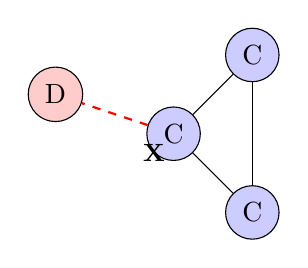
\begin{tikzpicture}
                    \node[draw, circle, fill=blue!20] (c1) at (0,0) {C};
                    \node[draw, circle, fill=blue!20] (c2) at (1,1) {C};
                    \node[draw, circle, fill=blue!20] (c3) at (1,-1) {C};
                    \node[draw, circle, fill=red!20] (d1) at (-1.5, 0.5) {D};
                    \draw (c1) -- (c2); \draw (c1) -- (c3); \draw (c2) -- (c3);
                    \draw[dashed, red, thick] (c1) -- (d1);
                    \node at (-0.25, -0.25) {\small \bf X};
                \end{tikzpicture}
                \captionof{figure}{[动态网络演化示意图]}
                
                \vspace{1cm}
                
                \includegraphics[width=\linewidth]{example-image-a}
                \captionof{figure}{[合作率演化对比图 (预期)]}
            \end{center}
        \end{column}
    \end{columns}
\end{frame}

\begin{frame}
    \frametitle{4.3 异质环境下的合作演化 (预期结果)}
     \begin{columns}
        \begin{column}{0.55\textwidth}
            \begin{itemize}
                \item \textbf{面对顽固背叛者：}
                \begin{itemize}
                    \item 少量顽固背叛者的存在会持续地对邻里环境造成破坏。
                    \item \textbf{预期：} NI学习者会通过社会学习，快速在其周围形成由合作者构成的“隔离带”或“防御工事”，将负面影响局部化。
                \end{itemize}
                \item \textbf{面对异质偏好：}
                \begin{itemize}
                    \item 群体中同时存在“功利主义者”（$w_P \approx 1$）和“声誉主义者”（$w_P \approx 0$）。
                    \item \textbf{预期：} NI机制可能会促进“同类相聚”，形成不同偏好智能体构成的社区，整个社会呈现出多样化的局部规范。
                \end{itemize}
            \end{itemize}
        \end{column}
        \begin{column}{0.4\textwidth}
            \begin{center}
                 \includegraphics[width=\linewidth]{example-image-b}
                 \captionof{figure}{[顽固背叛者周围的合作簇群 (预期)]}

                \vspace{1cm}
                 
                 \includegraphics[width=\linewidth]{example-image-c}
                 \captionof{figure}{[异质偏好下的社会分层 (预期)]}
            \end{center}
        \end{column}
    \end{columns}
\end{frame}

% ===============================
\section{总结与展望}
% ===============================
\begin{frame}
    \frametitle{5.1 全文工作总结}
    \begin{itemize}
        \item \textbf{理论创新：提出并验证了邻里感知 (NI) 社会学习机制}
        \begin{itemize}
            \item 系统性地证明了该机制在促进强化学习智能体达成合作方面的有效性，成功解释了合作簇群的形成。
            \item 揭示了其与声誉、感知范围等机制的强大协同效应。
        \end{itemize}
        \pause
        \item \textbf{稳健性检验：将模型扩展至复杂环境}
        \begin{itemize}
            \item 通过在动态网络和异质智能体环境中的扩展研究，初步探讨了 NI 机制在更真实场景下的适应性和稳健性。
        \end{itemize}
        \pause
        \item \textbf{研究贡献：}
        \begin{itemize}
            \item 为连接个体自适应学习、局部社会互动与宏观合作涌现提供了新的桥梁。
            \item 为设计促进大规模系统中合作行为的策略提供了理论参考。
        \end{itemize}
    \end{itemize}
\end{frame}

\begin{frame}
    \frametitle{5.2 未来工作展望}
    \begin{itemize}
        \item \textbf{模型层面：}
        \begin{itemize}
            \item 引入更复杂的强化学习算法，如深度强化学习 (DQN)，以处理更丰富的状态空间。
            \item 探索更多样化的网络拓扑结构，如小世界网络、无标度网络。
        \end{itemize}
        \item \textbf{机制层面：}
        \begin{itemize}
            \item 考虑信息的不确定性，如智能体只能观察到带噪声的邻居回报。
            \item 引入多样的社会学习规则，如不仅仅学习最好的，也避免最差的。
        \end{itemize}
        \item \textbf{应用层面：}
        \begin{itemize}
            \item 尝试将模型应用于解释具体的社会经济现象，如在线社区的规范形成。
        \end{itemize}
    \end{itemize}
\end{frame}


% --- Q&A ---
\begin{frame}
    \frametitle{} % No title for the thank you slide
    \begin{center}
        \Huge \textbf{感谢聆听，敬请批评指正！}
    \end{center}
\end{frame}

\end{document}
